% ELEC3607 Assignment 1 — WSPR-SDR Modifications
% Compile: pdflatex -> pdflatex (no BibTeX needed; references are inline)
% Images resolve from two directories via \graphicspath below.

\documentclass[conference]{IEEEtran}

\usepackage{cite}
\usepackage{amsmath,amssymb,amsfonts}
\usepackage{graphicx}
\usepackage{textcomp}
\usepackage{booktabs}
\usepackage{float}
\usepackage{listings}
\usepackage{xcolor}
\usepackage{hyperref}

% Image search paths: Part A pictures and the A1 root (Part B images)
\graphicspath{{PART_A/PartA_Pictures/}{./}}

\lstset{
  basicstyle=\ttfamily\scriptsize,
  breaklines=true,
  breakatwhitespace=false,
  language=bash,
  keywordstyle=\color{blue},
  commentstyle=\color{gray}\itshape,
  numbers=none,
  frame=single,
  framesep=2pt,
  xleftmargin=4pt,
  xrightmargin=4pt,
}
\lstdefinestyle{cstyle}{language=C, keywordstyle=\color{blue}}

% -------------------------------------------------------
\begin{document}

\title{WSPR-SDR Modifications: RF Loopback Transmitter and\\Shared-BPF Transceiver Design}

\author{
  \IEEEauthorblockN{Connor Nealis \ Rianne Joseph \ Muhammad Abdullah \ Sam (Sorry cannot remember last name and its not on whatsapp}
  \IEEEauthorblockA{
    School of Electrical and Information Engineering,
    University of Sydney, Sydney, Australia
  }
}

\maketitle

% -------------------------------------------------------
\begin{abstract}
This paper describes two modifications to a WSPR software-defined radio (SDR)
receiver built around the AUP-ZU3 FPGA platform. The first modification~(Part~A)
implements a 4-FSK WSPR transmitter using the Si5351A CLK2 output attenuated by
40~dB and injected into the receiver front end, demonstrating a complete
transmit--receive loopback at 7.040~MHz. The WSPR message \texttt{VK2AAR QF56 3~dBm}
was encoded as 162 4-FSK symbols and decoded at SNR\,=\,38~dB, confirming correct
encoder, frequency synthesis, and timing synchronisation. The second
modification~(Part~B) designs a hardware transceiver path: a BS170 MOSFET
common-source amplifier targeting 100~mW into 50~$\Omega$ at 7~MHz, and a
TI~TS5A23159 dual-channel analog switch that re-uses the existing 7~MHz bandpass
filter for both receive and transmit paths under GPIO control.
\end{abstract}

\begin{IEEEkeywords}
WSPR, SDR, Si5351A, 4-FSK, convolutional encoding, RF loopback, BS170,
common-source amplifier, T/R switch, bandpass filter
\end{IEEEkeywords}

% -------------------------------------------------------
\section{Introduction}

The WSPR-SDR is a 7~MHz weak-signal receiver designed to decode Weak Signal
Propagation Reporter (WSPR) transmissions---a 4-FSK mode with 1.4648~Hz tone
spacing capable of decoding signals as weak as $-28$~dB~SNR. The board interfaces
with an Avnet UltraZed-EG (AUP-ZU3) FPGA carrier running PetaLinux.

\textbf{Receive signal path.} An RF signal enters the 50~$\Omega$ SMA port (BPFIN)
and passes through a 7-element Chebyshev bandpass filter centred at 7~MHz. The
filtered signal feeds a Tayloe mixer (TI~TS3A5017 quad switch) driven by two
quadrature clocks---CLK0 and CLK1 from a Silicon Labs Si5351A on PLL\_A at
7.038600~MHz, 90$^\circ$ apart---producing in-phase and quadrature baseband
signals. A TL972 audio amplifier buffers the IQ outputs; these are captured by a
Plugable USB sound card at 48~kHz and piped via PulseAudio to the k9an-wsprd
decoder on the AUP-ZU3.

The Si5351A provides a third output, CLK2, on a separate PLL~(PLL\_B). In the
unmodified receiver CLK2 is unused. Part~A re-purposes CLK2 as a
software-controlled WSPR transmitter; Part~B adds dedicated hardware for a full
transceiver capability. Both modifications are described in the sections that
follow; this paper is self-contained and does not assume familiarity with the
original WSPR-SDR design.

% -------------------------------------------------------
\section{Part A: WSPR RF Loopback Transmitter}

\subsection{Hardware Modification}

The CLK2 output (Si5351A, PLL\_B) produces a 3.3~V LVCMOS square wave at
$\approx$7.040~MHz with an equivalent output power of $\approx$0~dBm into
50~$\Omega$. The receiver front end is designed for over-the-air signals in the
$-100$ to $-70$~dBm range; direct connection would overdrive the mixer and amplifier
by 70--100~dB. Two SMA barrel attenuators (ATT1~=~20~dB, ATT2~=~20~dB) were
connected in series between the CLK2 test point~(TP6) and the BPFIN SMA connector,
as shown in Fig.~\ref{fig:loopback_schem} and Fig.~\ref{fig:pcb}. Total
attenuation is 40~dB:
%
\begin{equation}
  P_\text{BPFIN} = P_\text{CLK2} - 40\,\text{dB}
                 = 0\,\text{dBm} - 40\,\text{dB} = -40\,\text{dBm}
  \label{eq:atten}
\end{equation}
%
This places the injected signal at $-40$~dBm (100~nW), well within the front-end
linear range while providing a high-SNR loopback for verification.

\begin{figure}[t]
  \centering
  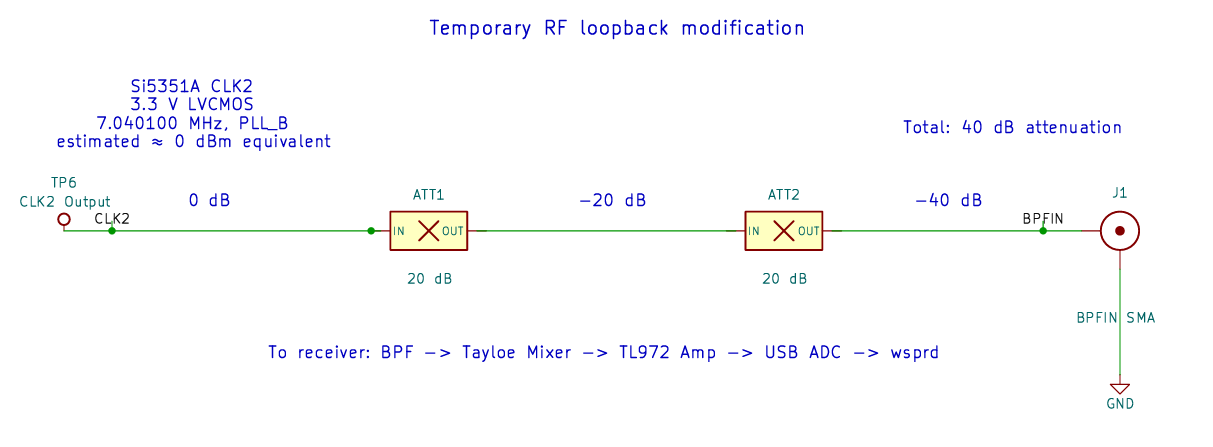
\includegraphics[width=\columnwidth]{SimpleschematicPartA}
  \caption{RF loopback schematic. CLK2~(TP6, $\approx$0~dBm) drives two cascaded
           20~dB SMA attenuators for 40~dB total attenuation, injecting
           $-40$~dBm into the BPFIN port. Signal then traverses the existing
           receive chain: BPF $\to$ Tayloe mixer $\to$ TL972 amp $\to$
           USB ADC $\to$ wsprd.}
  \label{fig:loopback_schem}
\end{figure}

\begin{figure}[t]
  \centering
  \includegraphics[width=\columnwidth]{IMG_0656}
  \caption{Modified hardware. The AUP-ZU3 FPGA board~(top) connects to the
           WSPR-SDR daughter board~(bottom right) via ribbon cable. The 40~dB
           SMA attenuator chain~(left) bridges CLK2 TP6 to the BPFIN SMA
           connector.}
  \label{fig:pcb}
\end{figure}

\subsection{WSPR Encoder --- \texttt{wspr\_encode.c}}

The WSPR protocol encodes a callsign, 4-character Maidenhead locator, and
transmit power level into 162 4-FSK symbols through five stages.

\textbf{Stage~1 --- Callsign packing (28~bits).} The callsign is normalised to
six characters and encoded as a mixed-radix integer:
%
\begin{align}
  N = &\; c_0 \cdot 36 \cdot 10 \cdot 27^3
      + c_1 \cdot 10 \cdot 27^3
      + c_2 \cdot 27^3 \notag \\
      &+ (c_3{-}10) \cdot 27^2
      + (c_4{-}10) \cdot 27
      + (c_5{-}10)
  \label{eq:callsign}
\end{align}
%
where $c_0\!\in\![0,36]$ (alphanumeric~+~space), $c_1\!\in\![0,35]$,
$c_2\!\in\![0,9]$ (digit only), and $c_{3\text{--}5}\!\in\![10,36]$ (alpha only).
\textit{(wspr\_encode.c L57--L92)}

\textbf{Stage~2 --- Grid and power packing (22~bits).}
%
\begin{align}
  M &= \bigl(179 - 10(l_0{-}\texttt{'A'}) - (l_2{-}\texttt{'0'})\bigr)\cdot 180
       + 10(l_1{-}\texttt{'A'}) + (l_3{-}\texttt{'0'}) \notag \\
    & \leftarrow M \cdot 128 + P_\text{dBm} + 64
  \label{eq:grid}
\end{align}
%
\textit{(wspr\_encode.c L98--L109)}

\textbf{Stage~3 --- 50-bit packing.} $N$~(28~bits) and $M$~(22~bits) are
concatenated and zero-padded to 81~bits for the convolutional encoder.
\textit{(L115--L123)}

\textbf{Stage~4 --- Convolutional FEC (rate~$\frac{1}{2}$, $K$=32).} Each input
bit is shifted through a 32-bit register; two parity bits are generated using
generator polynomials \texttt{0xF2D05351} and \texttt{0xE4613C47}, yielding
162~coded bits. The rate-$\frac{1}{2}$ code enables the $-28$~dB~SNR decoding
floor. \textit{(L129--L146)}

\textbf{Stage~5 --- Interleaving and sync vector.} The 162~coded bits are
permuted by an 8-bit bit-reversal interleaver, then merged with the 162-bit
pseudo-random sync vector:
%
\begin{equation}
  \texttt{symbol}[i]
    = \texttt{SYNC\_VECTOR}[i] + 2 \times \texttt{interleaved}[i]
  \label{eq:sync}
\end{equation}
%
producing 162 symbols $\in \{0,1,2,3\}$ (the 4-FSK alphabet).
\textit{(L179--L203)}

Encoder correctness was verified by comparing the output for
\texttt{VK2AAX QF56 37} against a reference Python encoder; all 162~symbols
matched exactly.

\subsection{Transmitter --- \texttt{wspr\_transmit.c}}

CLK2 uses PLL\_B independently so frequency changes do not disturb the receiver
LO on PLL\_A. The clock frequency plan is given in Table~\ref{tab:clocks}.

\begin{table}[t]
  \centering
  \caption{Si5351A Clock Frequency Plan}
  \label{tab:clocks}
  \begin{tabular}{llll}
    \toprule
    Clock & PLL & Frequency & Role \\
    \midrule
    CLK0 & PLL\_A & 7.038600~MHz       & Rx LO (I) \\
    CLK1 & PLL\_A & 7.038600~MHz, 90°  & Rx LO (Q) \\
    CLK2 & PLL\_B & 7.040100--7.040104~MHz & Tx \\
    \bottomrule
  \end{tabular}
\end{table}

\textbf{Frequency offset rationale.} If CLK2 matched the LO frequency, the Tayloe
mixer would produce a DC output. The transmitter must be offset so that the mixer
produces an audio tone at 1500~Hz---the centre of the k9an-wsprd decoder's search
window:
%
\begin{equation}
  f_\text{audio} = f_\text{TX} - f_\text{LO}
                 = 7{,}040{,}100 - 7{,}038{,}600 = 1{,}500\,\text{Hz}
  \label{eq:offset}
\end{equation}

\textbf{PLL\_B register calculation (AN619).} For each tone frequency $f_k$, the
VCO is set to $f_\text{VCO} = f_k \times N$ with integer divider $N=126$. The
feedback multiplier $M = f_\text{VCO}/f_\text{xtal}$ is decomposed with
denominator $c = 1{,}000{,}000$:
%
\begin{lstlisting}[style=cstyle,language=C]
a = (int)floor(M);
b = (int)round((M - a) * c);
P1 = 128*a + (int)floor(128.0*b/c) - 512;
P2 = 128*b - c*(int)floor(128.0*b/c);
P3 = c;   // write P1,P2,P3 to regs 0x22-0x29 via I2C
\end{lstlisting}
%
\textit{(wspr\_transmit.c L185--L221)}

\textbf{Tone spacing accuracy.} WSPR specifies a tone spacing of
$12000/8192 = 1.4648$~Hz. With the Si5351A minimum frequency step
$\Delta f_\text{min} = 27{,}000{,}000 / (1{,}000{,}000 \times 126) = 0.214$~Hz,
the nearest achievable spacing is $7 \times 0.214 = 1.500$~Hz---a 2.4\% error,
verified to be within the decoder's tolerance. The four achieved tone frequencies
are shown in Table~\ref{tab:tones}.

\begin{table}[t]
  \centering
  \caption{Tone Frequencies (MS2\_div=126, denom=1\,000\,000)}
  \label{tab:tones}
  \begin{tabular}{cccc}
    \toprule
    Tone & Target (Hz) & Actual (Hz) & Error (Hz) \\
    \midrule
    0 & 7\,040\,100.000 & 7\,040\,100.000 & $+$0.0000 \\
    1 & 7\,040\,101.465 & 7\,040\,101.500 & $+$0.0352 \\
    2 & 7\,040\,102.930 & 7\,040\,103.000 & $+$0.0703 \\
    3 & 7\,040\,104.395 & 7\,040\,104.500 & $+$0.1055 \\
    \bottomrule
  \end{tabular}
\end{table}

\textbf{Transmission loop.} For each of the 162~symbols the PLL\_B registers are
updated (8~I$^2$C writes) then the CPU sleeps for one symbol period:
%
\begin{lstlisting}[style=cstyle,language=C]
for (i = 0; i < 162; i++) {
    si5351_set_pllb(&tones[symbols[i]]);
    nanosleep(682667 /* us */);
}
// Total: 162 x 682.667 ms = 110.6 s
\end{lstlisting}
%
\textit{(wspr\_transmit.c L486--L511)}

The transmitter waits for an even UTC minute boundary before starting, synchronised
with the \texttt{wsprwait} decoder script, ensuring the 114-second recording window
captures the full 110.6-second transmission.
\textit{(wspr\_transmit.c L307--L347)}

\subsection{Software Setup}

The following commands bring up the complete transmit--receive system. They are run
across two terminals on the AUP-ZU3.

\begin{lstlisting}
# T2: program Si5351A (CLK0/CLK1 for Rx LO; CLK2 disabled)
cd si5351/ && sudo ./i2cread

# T2: set USB sound card as PulseAudio source
pactl set-default-source \
  alsa_input.usb-Plugable_...-00.analog-stereo
# keep card active (prevents PulseAudio suspend)
parec --device=alsa_input.usb-Plugable_... \
  > /dev/null &

# T2: start decoder (syncs to next even UTC minute)
./wsprwait

# T1: transmit (run simultaneously with decoder)
sudo ./wspr_transmit VK2AAR QF56 3
\end{lstlisting}

The \texttt{parec} background process is essential: PulseAudio suspends an idle
capture device after a few seconds, causing the decoder to record silence.

\subsection{Results}

Two consecutive decode runs are presented. In both, \texttt{VK2AAR QF56 3} was
recovered correctly.

\begin{figure}[t]
  \centering
  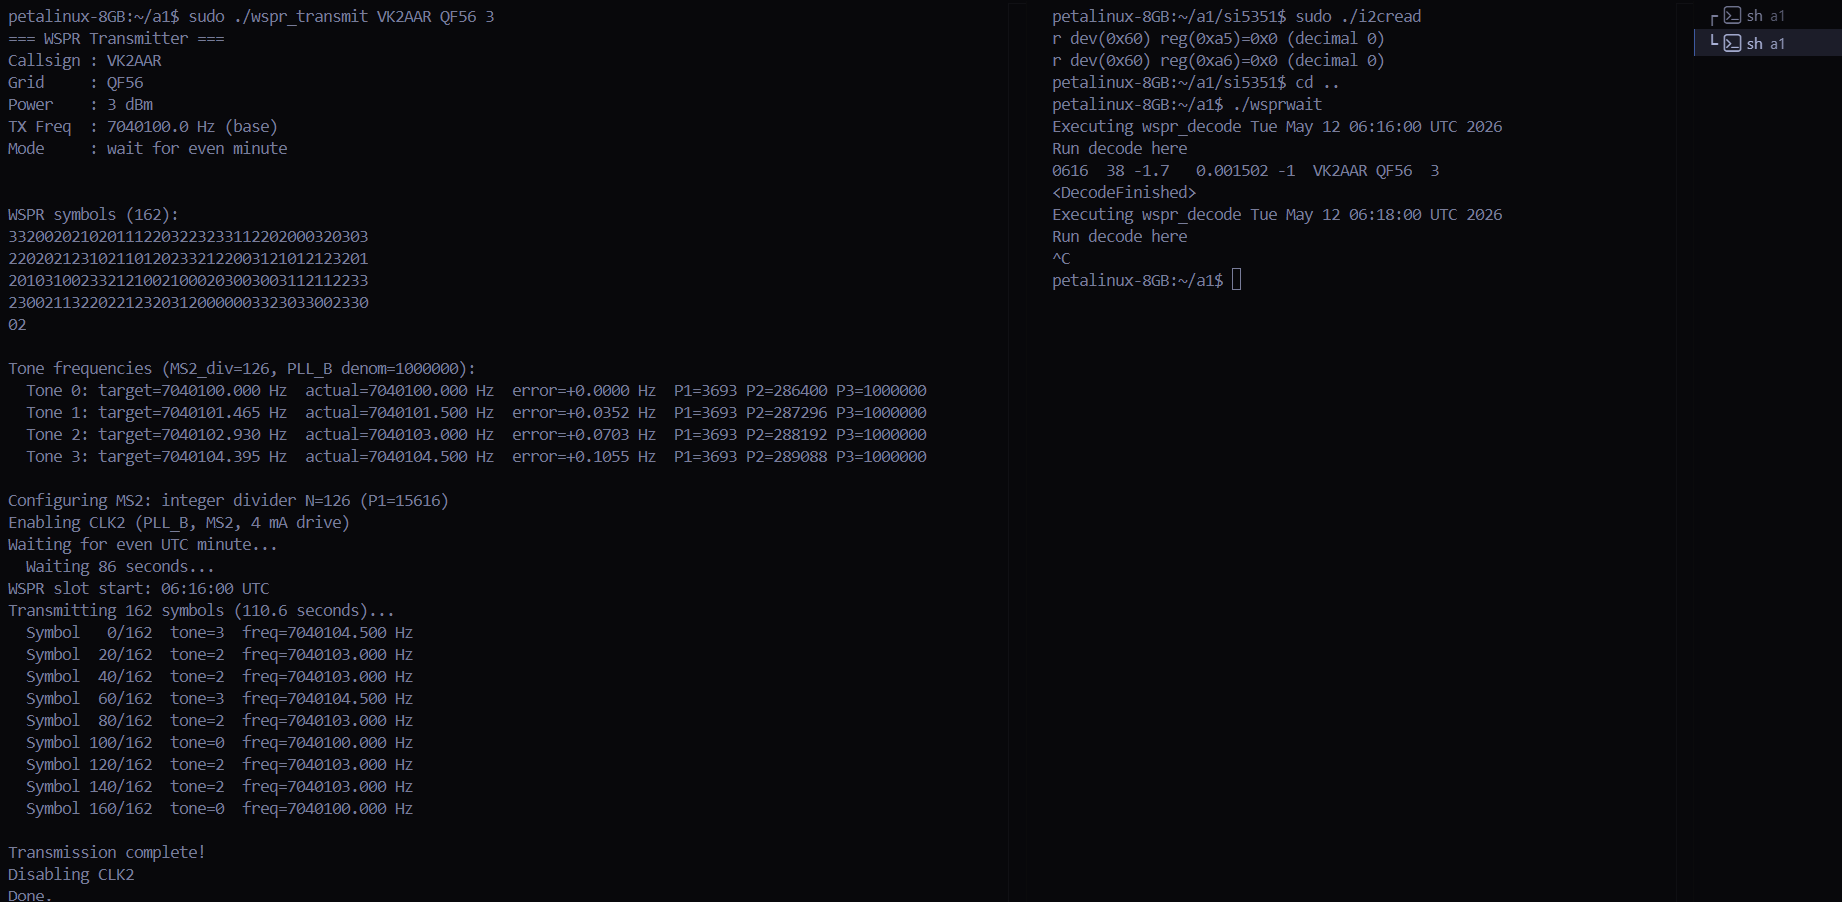
\includegraphics[width=\columnwidth]{SplitTerminal}
  \caption{First loopback decode (06:16:00~UTC). Left: transmitter output showing
           162-symbol schedule and ``Transmission complete.'' Right: decoder
           confirming SNR\,=\,38~dB, offset~$-1.7$~ppm, audio
           frequency~1502~Hz.}
  \label{fig:decode1}
\end{figure}

\begin{figure}[t]
  \centering
  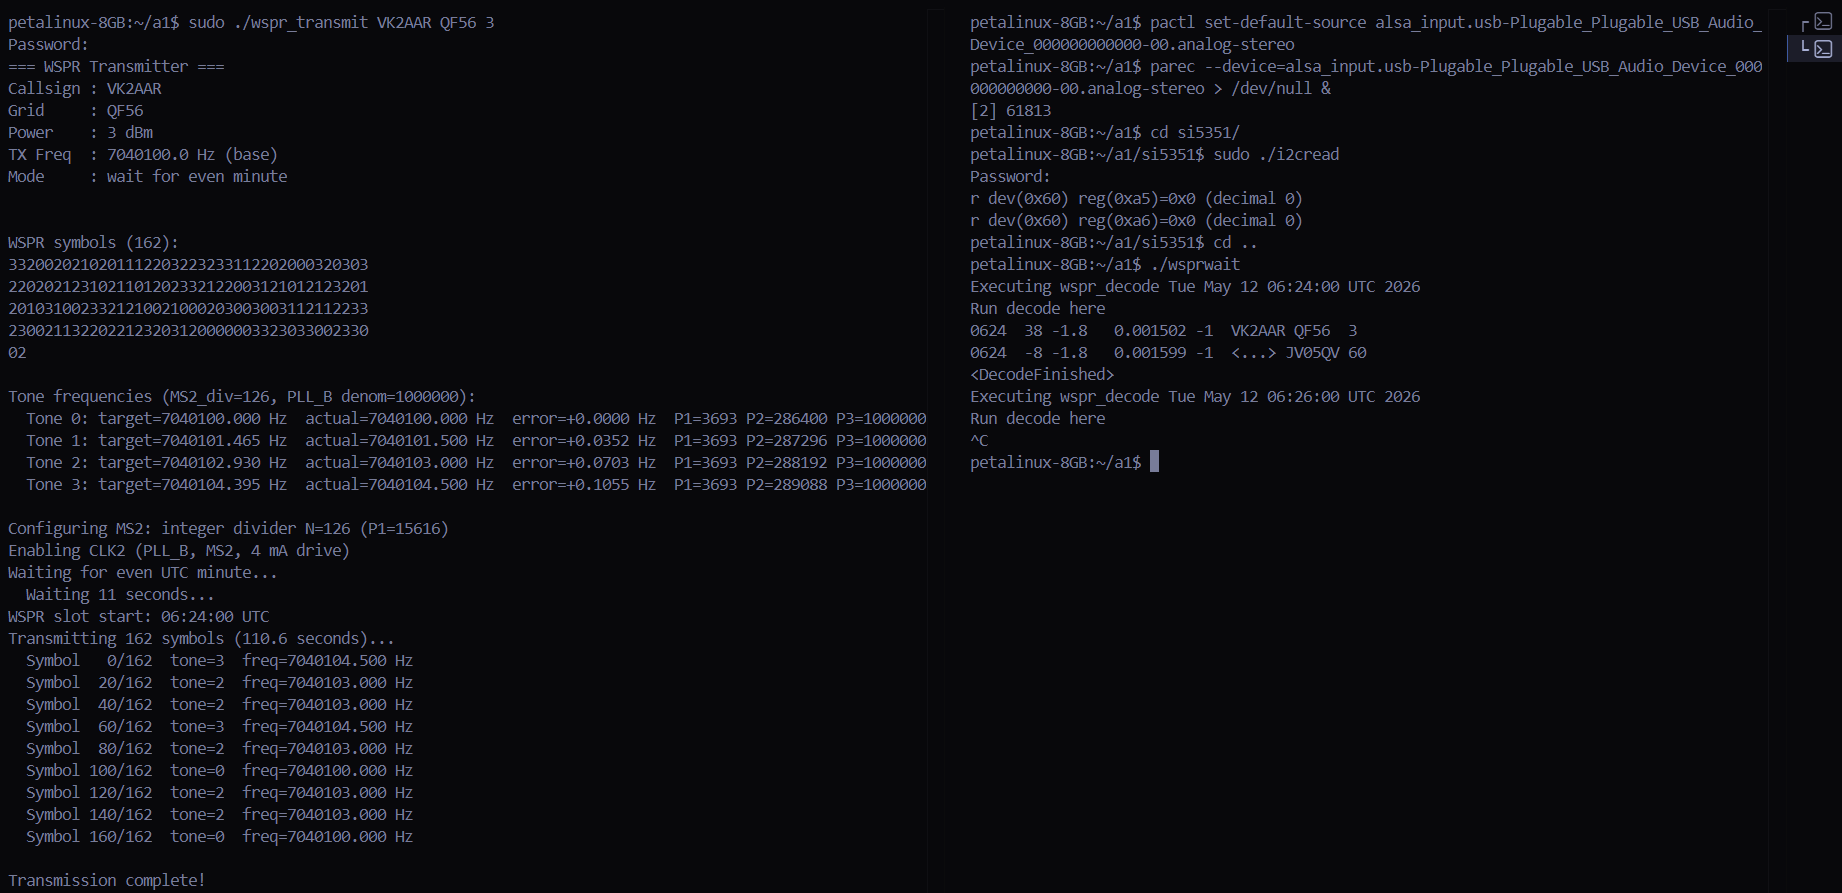
\includegraphics[width=\columnwidth]{Split2}
  \caption{Second loopback decode (06:24:00~UTC). Primary decode: SNR\,=\,38~dB,
           $-1.8$~ppm. Spurious decode (\texttt{JV05QV~60}) is a statistical
           artefact of the convolutional search; normal behaviour at high SNR.}
  \label{fig:decode2}
\end{figure}

\begin{table}[t]
  \centering
  \caption{Loopback Decode Results}
  \label{tab:results}
  \begin{tabular}{ccccc}
    \toprule
    UTC Slot & SNR (dB) & Offset (ppm) & $f_\text{audio}$ (Hz) & Message \\
    \midrule
    06:16 & 38 & $-1.7$ & 1502 & VK2AAR QF56 3 \\
    06:24 & 38 & $-1.8$ & 1502 & VK2AAR QF56 3 \\
    \bottomrule
  \end{tabular}
\end{table}

Table~\ref{tab:results} summarises both runs. The 38~dB SNR is expected for a
direct RF connection; over-the-air signals from the lab beacon VK2APL were received
at $-7$ to $-14$~dB~SNR. The decoded audio frequency (1502~Hz) is within 2~Hz of
the 1500~Hz design target~\eqref{eq:offset}.

% -------------------------------------------------------
\section{Part B: Transmit Amplifier and Shared-BPF Path}

\subsection{Design Objectives}

Part~B converts the receiver into a hardware transceiver by adding: (1)~a transmit
power amplifier delivering 100~mW into 50~$\Omega$ at 7~MHz from the CLK2 input,
and (2)~a T/R switching network re-using the existing 7~MHz BPF for both signal
paths under GPIO control.

\subsection{Transmit Amplifier}

% TODO: write amplifier design equations and explanation.
% Key figures available:
%   tx_specs.png            -- amplifier specifications / design target
%   tx_input_voltage_clk2.png -- CLK2 input waveform
%   tx_amplifier.png        -- BS170 common-source schematic
%   tx_output_rf.png        -- output waveform at 7 MHz

\begin{figure}[t]
  \centering
  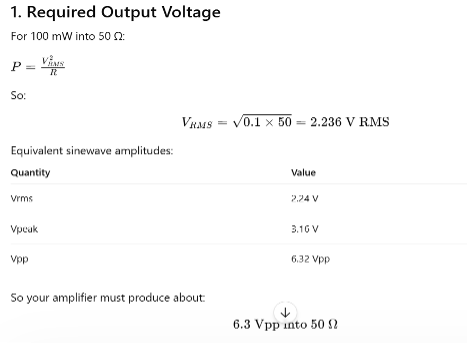
\includegraphics[width=\columnwidth]{tx_specs}
  \caption{Tx amplifier design specification.}
  \label{fig:tx_specs}
\end{figure}

\begin{figure}[t]
  \centering
  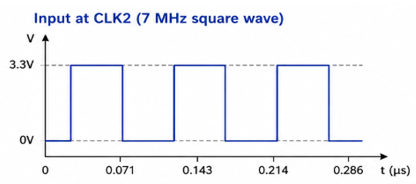
\includegraphics[width=0.8\columnwidth]{tx_input_voltage_clk2}
  \caption{CLK2 input signal: 0--3.3~V square wave at $\approx$7~MHz driving
           the BS170 gate.}
  \label{fig:clk2_input}
\end{figure}

\begin{figure}[t]
  \centering
  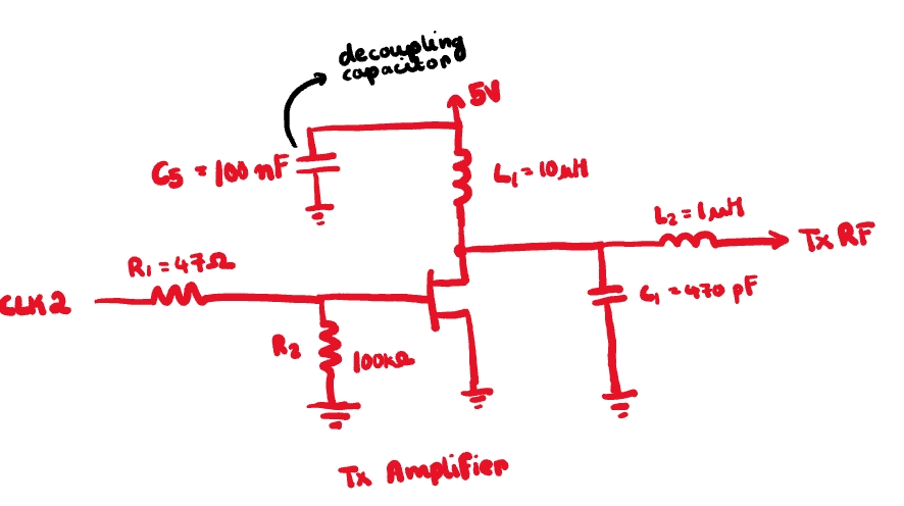
\includegraphics[width=\columnwidth]{tx_amplifier}
  \caption{BS170 common-source transmit amplifier schematic. Resonant drain
           tank (L1, L2, C1) tuned to 7~MHz; 5~V supply; C5~=~100~nF decoupling;
           50~$\Omega$ SMA load (BWSMA-KE-P001).}
  \label{fig:tx_amp}
\end{figure}

\begin{figure}[t]
  \centering
  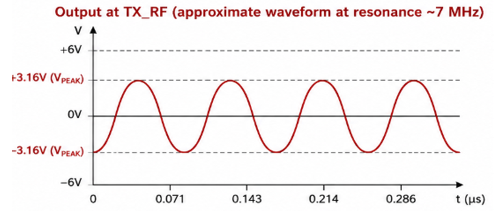
\includegraphics[width=0.8\columnwidth]{tx_output_rf}
  \caption{Tx amplifier output waveform at 7~MHz ($\approx$6.3~V$_\text{pp}$
           into 50~$\Omega$, corresponding to $\approx$100~mW).}
  \label{fig:tx_output}
\end{figure}

\subsection{T/R Switching Network}

% TODO: write switching network explanation.
% Key figures available:
%   tssa231259.png          -- TS5A23159 component / package
%   functional_diagram_ts.png -- TS5A23159 functional block diagram
%   functional_table_ts.png -- truth table (IN=0: COM-NC, IN=1: COM-NO)
%   schem.png               -- full T/R switch + amplifier KiCad schematic
%   pcb_schem.png           -- KiCad PCB layout
%   Unbenannt.png           -- (identify and caption)

\begin{figure}[t]
  \centering
  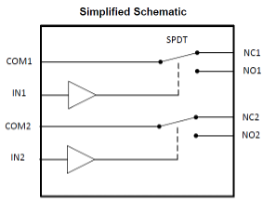
\includegraphics[width=0.7\columnwidth]{functional_diagram_ts}
  \caption{TS5A23159 dual-channel analog switch functional diagram.}
  \label{fig:ts_func}
\end{figure}

\begin{figure}[t]
  \centering
  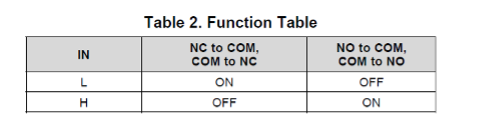
\includegraphics[width=0.7\columnwidth]{functional_table_ts}
  \caption{TS5A23159 truth table. GPIO23\,=\,0: COM connects to NC (Rx path);
           GPIO23\,=\,1: COM connects to NO (Tx path).}
  \label{fig:ts_table}
\end{figure}

\begin{figure}[t]
  \centering
  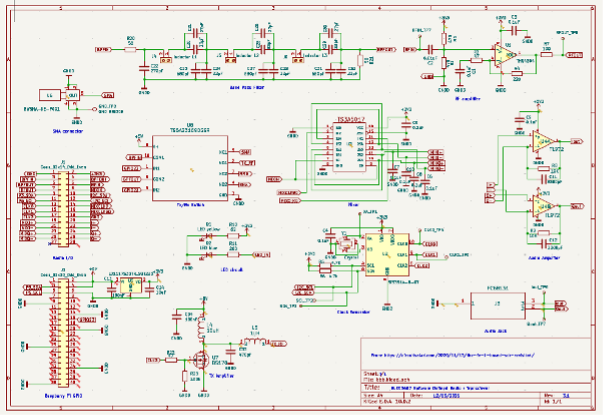
\includegraphics[width=\columnwidth]{schem}
  \caption{Full KiCad schematic: BS170 Tx amplifier and TS5A23159 T/R switching
           network integrated with the existing WSPR-SDR BPF and LNA.}
  \label{fig:full_schem}
\end{figure}

\begin{figure}[t]
  \centering
  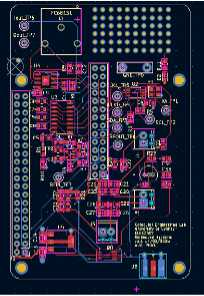
\includegraphics[width=\columnwidth]{pcb_schem}
  \caption{KiCad PCB layout. New components (Tx amplifier, analog switch)
           placed and routed alongside the existing WSPR-SDR board.}
  \label{fig:pcb_layout}
\end{figure}

% -------------------------------------------------------
\section{Conclusion}

Part~A demonstrated a complete WSPR transmit--receive loopback: CLK2 was attenuated
40~dB and injected into BPFIN, and the message \texttt{VK2AAR QF56 3} was decoded
in two consecutive runs at SNR\,=\,38~dB with an audio frequency of 1502~Hz,
confirming correct encoder operation, PLL\_B frequency synthesis, and
UTC-synchronised timing. Part~B designed a hardware transceiver upgrade: a BS170
common-source amplifier targeting 100~mW at 7~MHz and a TS5A23159 dual-channel
switch enabling the existing BPF to serve both Rx and Tx paths under single-GPIO
control, with KiCad schematics and PCB layout ready for fabrication.

% -------------------------------------------------------
\begin{thebibliography}{6}

\bibitem{si5351ds}
Silicon Laboratories, ``Si5351A/B/C-B I$^2$C Clock Generator,'' Datasheet
Rev.~1.3, 2018.

\bibitem{an619}
Silicon Laboratories, ``AN619: Manually Generating an Si5351 Register Map,''
Application Note Rev.~0.3, 2016.

\bibitem{ts5a}
Texas Instruments, ``TS5A23159 Dual-Channel 1-$\Omega$ SPDT Analog Switch,''
SCDS139C, 2004.

\bibitem{bs170}
ON Semiconductor, ``BS170 N-Channel Enhancement Mode Field Effect Transistor,''
Datasheet Rev.~4, 2014.

\bibitem{wsprd}
K.~Fleisher (k9an), ``wsprd WSPR Decoder,'' [Software].
Available: \url{https://github.com/k9an/wsprd}

\bibitem{qex}
J.~Ahlstrom, ``An All-Digital Transceiver for HF,'' \textit{QEX},
pp.~1--6, Nov./Dec. 2010.

\end{thebibliography}

% -------------------------------------------------------
\appendix

\section{wspr\_encode.c --- FEC and Symbol Generation}
\label{app:encode}

\begin{lstlisting}[style=cstyle,language=C]
/* Stage 4: convolutional FEC, rate 1/2, K=32 */
#define POLY1 0xF2D05351
#define POLY2 0xE4613C47

for (i = 0; i < 81; i++) {
    reg = (reg << 1) | input_bit[i];
    coded[2*i]   = parity32(reg & POLY1);
    coded[2*i+1] = parity32(reg & POLY2);
}

/* Stage 5: interleave + sync merge */
for (i = 0; i < 162; i++)
    symbol[i] = SYNC_VECTOR[i] + 2 * interleaved[i];
\end{lstlisting}

Full source: \texttt{PART\_A/CODE.zip} --- \texttt{wspr\_encode.c}

\section{wspr\_transmit.c --- PLL\_B Register Write}
\label{app:transmit}

\begin{lstlisting}[style=cstyle,language=C]
/* AN619 decomposition; c = 1,000,000 */
a  = (int)floor(M);
b  = (int)round((M - a) * c);
P1 = 128*a + (int)floor(128.0*b/c) - 512;
P2 = 128*b - c*(int)floor(128.0*b/c);
P3 = c;
/* Write P1,P2,P3 to Si5351A regs 0x22-0x29 via I2C */
\end{lstlisting}

Full source: \texttt{PART\_A/CODE.zip} --- \texttt{wspr\_transmit.c}

\end{document}
